% Taken from: https://mikedewar.wordpress.com/2009/02/25/latex-beamer-python-beauty/
\documentclass[12pt,english,pdf,xcolor=dvipsnames,aspectratio=169,handout]{beamer}\usepackage[]{graphicx}\usepackage[]{xcolor}
% maxwidth is the original width if it is less than linewidth
% otherwise use linewidth (to make sure the graphics do not exceed the margin)
\makeatletter
\def\maxwidth{ %
  \ifdim\Gin@nat@width>\linewidth
    \linewidth
  \else
    \Gin@nat@width
  \fi
}
\makeatother

\definecolor{fgcolor}{rgb}{0.345, 0.345, 0.345}
\newcommand{\hlnum}[1]{\textcolor[rgb]{0.686,0.059,0.569}{#1}}%
\newcommand{\hlstr}[1]{\textcolor[rgb]{0.192,0.494,0.8}{#1}}%
\newcommand{\hlcom}[1]{\textcolor[rgb]{0.678,0.584,0.686}{\textit{#1}}}%
\newcommand{\hlopt}[1]{\textcolor[rgb]{0,0,0}{#1}}%
\newcommand{\hlstd}[1]{\textcolor[rgb]{0.345,0.345,0.345}{#1}}%
\newcommand{\hlkwa}[1]{\textcolor[rgb]{0.161,0.373,0.58}{\textbf{#1}}}%
\newcommand{\hlkwb}[1]{\textcolor[rgb]{0.69,0.353,0.396}{#1}}%
\newcommand{\hlkwc}[1]{\textcolor[rgb]{0.333,0.667,0.333}{#1}}%
\newcommand{\hlkwd}[1]{\textcolor[rgb]{0.737,0.353,0.396}{\textbf{#1}}}%
\let\hlipl\hlkwb

\usepackage{framed}
\makeatletter
\newenvironment{kframe}{%
 \def\at@end@of@kframe{}%
 \ifinner\ifhmode%
  \def\at@end@of@kframe{\end{minipage}}%
  \begin{minipage}{\columnwidth}%
 \fi\fi%
 \def\FrameCommand##1{\hskip\@totalleftmargin \hskip-\fboxsep
 \colorbox{shadecolor}{##1}\hskip-\fboxsep
     % There is no \\@totalrightmargin, so:
     \hskip-\linewidth \hskip-\@totalleftmargin \hskip\columnwidth}%
 \MakeFramed {\advance\hsize-\width
   \@totalleftmargin\z@ \linewidth\hsize
   \@setminipage}}%
 {\par\unskip\endMakeFramed%
 \at@end@of@kframe}
\makeatother

\definecolor{shadecolor}{rgb}{.97, .97, .97}
\definecolor{messagecolor}{rgb}{0, 0, 0}
\definecolor{warningcolor}{rgb}{1, 0, 1}
\definecolor{errorcolor}{rgb}{1, 0, 0}
\newenvironment{knitrout}{}{} % an empty environment to be redefined in TeX

\usepackage{alltt}
\usepackage{etex}
\usetheme{default}
\beamertemplatenavigationsymbolsempty
\definecolor{fore}{RGB}{43,41,46}
\definecolor{back}{RGB}{255,255,255}
\definecolor{title}{RGB}{198,24,38}
\setbeamercolor{titlelike}{fg=title}
\setbeamercolor{normal text}{fg=fore,bg=back}
\usepackage{mathpazo}
\usepackage{amsmath}
\usepackage{multirow}
\renewcommand{\familydefault}{\rmdefault}
\usepackage[T1]{fontenc}
\usepackage{inputenc}
\usepackage{parskip}
\setcounter{secnumdepth}{3}
\setcounter{tocdepth}{3}
\usepackage{hyperref}
\hypersetup{pdfauthor={Constantin Manuel Bosancianu},
pdftitle={Advanced Topics in Applied Regression},
pdfsubject={Day 5: Robust Regression},
pdfkeywords={Budapest, ECPR, 2017, day 5, SSMT}}
\usepackage{babel}
\usepackage{graphicx}
\usepackage{subfigure}
\usepackage{palatino}
% Defines a checkmark
\def\checkmark{\tikz\fill[scale=0.4,color=title](0,.35) -- (.25,0) -- (1,.7) -- (.25,.15) -- cycle;}
\setbeamertemplate{itemize items}{\checkmark}
% For table captions in Beamer
\usepackage[labelformat=empty]{caption}
\captionsetup[figure]{labelfont={color=fore}}
\captionsetup[table]{labelfont={color=fore}}
\usepackage{tikz, tikz-cd, animate}
\usetikzlibrary{shapes,backgrounds,trees}
\usetikzlibrary{decorations.pathreplacing}
\usepackage{pgfplots}
\pgfplotsset{compat=1.10}
\usepgfplotslibrary{fillbetween}
\usepackage{pgfplotstable}
\usepackage{wrapfig}
\usepackage{booktabs}
\usepackage{dcolumn}
\usepackage[sectionbib]{apacite}
\renewcommand{\bibliographytypesize}{\footnotesize}
% Set the design of the footer
\makeatletter
\setbeamercolor{author in head/foot}{fg=white, bg=title}
\setbeamercolor{date in head/foot}{fg=white, bg=title}
\setbeamercolor{institute in head/foot}{fg=white, bg=title}
\setbeamertemplate{footline}
{
  \leavevmode%
  \hbox{%
  \begin{beamercolorbox}[wd=.3333333\paperwidth,ht=2.25ex,dp=1ex,center]{author in head/foot}%
    \usebeamerfont{author in head/foot}\insertauthor
  \end{beamercolorbox}%
    \begin{beamercolorbox}[wd=.3333333\paperwidth,ht=2.25ex,dp=1ex,center]{institute in head/foot}%
    \usebeamerfont{institute in head/foot}Central European University, Budapest
  \end{beamercolorbox}%
  \begin{beamercolorbox}[wd=.3333333\paperwidth,ht=2.25ex,dp=1ex,right]{date in head/foot}%
    \usebeamerfont{date in head/foot}\insertshortdate{}\hspace*{2em}
    \insertframenumber{} / \inserttotalframenumber\hspace*{2ex}
  \end{beamercolorbox}}%
  \vskip0pt%
}
\makeatother
\title{Advanced Topics in Applied Regression}
\subtitle{Day 5: Robust regression}
\author{Constantin Manuel Bosancianu}
\institute{Doctoral School of Political Science \\ Central European University, Budapest\\\href{mailto:bosancianu@icloud.com}{bosancianu@icloud.com}}
\date{August 4, 2017}
\IfFileExists{upquote.sty}{\usepackage{upquote}}{}
\begin{document}
\maketitle
% PREAMBLE %




\section{Preamble: Detecting Influential Observations}

\begin{frame}{Perils of outliers}

\begin{figure}
\centering
\includegraphics[scale=0.45]{../04-graphs/05-05}
\caption{\textit{American Sociological Review}: frequency decreases with marital duration and age; some period effects are also found, related to risks of contraceptive use. $N=2062$.}
\end{figure}

\end{frame}


\begin{frame}{Perils of outliers}

\begin{figure}
\centering
\includegraphics[scale=0.45]{../04-graphs/05-06}
\caption{\textit{American Sociological Review}: removing 8 cases makes age effects disappear; estimating model on marriages $>2\; yrs$ (88 \% of sample) makes age, duration and period effects disappear.}
\end{figure}

\end{frame}



\begin{frame}{Perils of outliers}

\begin{figure}
\centering
\includegraphics[scale=0.40]{../04-graphs/05-07}
\caption{\textit{American Sociological Review}: removing cases leads to sample truncation and an unwarranted reduction in variance in the outcome.}
\end{figure}

\end{frame}

\begin{frame}[fragile]{Outliers and high leverage cases}

\begin{figure}
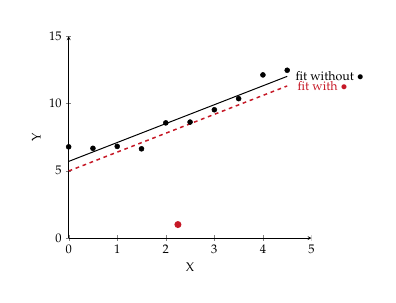
\begin{tikzpicture}[scale=0.45]
% For the regression graph below
\pgfmathsetseed{1146} % set the random seed
\pgfplotstableset{ % Define the equations for x and y
	create on use/x/.style={create col/expr={\pgfplotstablerow/2}},
	create on use/y/.style={create col/expr={1.3*\thisrow{x} + 5.5 + 1.5*rand}}
}
% create a new table with 10 rows and columns x and y:
\pgfplotstablenew[columns={x,y}]{10}\loadedtable
\begin{axis}[
xlabel=X, % label x axis
ylabel=Y, % label y axis
axis lines=left, %set the position of the axes
xmin=0, xmax=5, % set the min and max values of the x-axis
ymin=0, ymax=15, % set the min and max values of the y-axis
clip=false
]

%\pgfplotstablesave{\loadedtable}{../05-tables/Tab09.dat}

\addplot [only marks] table {\loadedtable};
\addplot [no markers, thick, title] table [y={create col/linear regression={y=y}}] {\loadedtable} node[xshift=1.2cm] {fit without $\bullet$};
\node [circle, fill=title, color=title, inner sep=-2pt] (A) at (225,10) {};
\draw[very thick, dashed, color=title] (0, 49.80074)--(450,113.05366) node[xshift=1cm] {fit with $\bullet$}; 
\end{axis}
\end{tikzpicture}
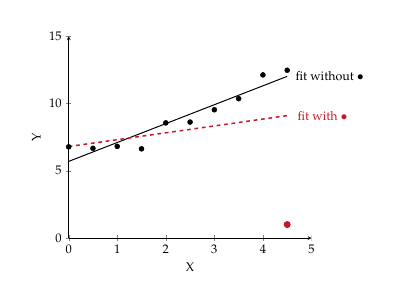
\begin{tikzpicture}[scale=0.45]
% For the regression graph below
\pgfmathsetseed{1146} % set the random seed
\pgfplotstableset{ % Define the equations for x and y
	create on use/x/.style={create col/expr={\pgfplotstablerow/2}},
	create on use/y/.style={create col/expr={1.3*\thisrow{x} + 5.5 + 1.5*rand}}
}
% create a new table with 10 rows and columns x and y:
\pgfplotstablenew[columns={x,y}]{10}\loadedtable
\begin{axis}[
xlabel=X, % label x axis
ylabel=Y, % label y axis
axis lines=left, %set the position of the axes
xmin=0, xmax=5, % set the min and max values of the x-axis
ymin=0, ymax=15, % set the min and max values of the y-axis
clip=false
]

\addplot [only marks] table {\loadedtable};
\addplot [no markers, thick, title] table [y={create col/linear regression={y=y}}] {\loadedtable} node[xshift=1.2cm] {fit without $\bullet$};
\node [circle, fill=title, color=title, inner sep=-2pt] (A) at (450,10) {};
\draw[very thick, dashed, color=title] (0, 68,857)--(450,91,90272) node[xshift=1cm] {fit with $\bullet$}; 
\end{axis}
\end{tikzpicture}
\centering
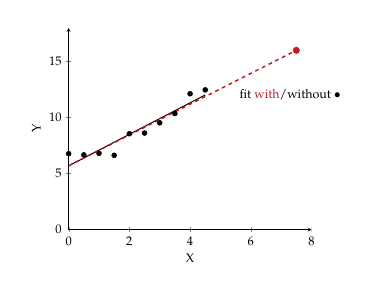
\begin{tikzpicture}[scale=0.45]
% For the regression graph below
\pgfmathsetseed{1146} % set the random seed
\pgfplotstableset{ % Define the equations for x and y
	create on use/x/.style={create col/expr={\pgfplotstablerow/2}},
	create on use/y/.style={create col/expr={1.3*\thisrow{x} + 5.5 + 1.5*rand}}
}
% create a new table with 10 rows and columns x and y:
\pgfplotstablenew[columns={x,y}]{10}\loadedtable
\begin{axis}[
xlabel=X, % label x axis
ylabel=Y, % label y axis
axis lines=left, %set the position of the axes
xmin=0, xmax=8, % set the min and max values of the x-axis
ymin=0, ymax=18, % set the min and max values of the y-axis
clip=false
]

\addplot [only marks] table {\loadedtable};
\addplot [no markers, thick, title] table [y={create col/linear regression={y=y}}] {\loadedtable} node[xshift=2.4cm] {fit \textcolor{title}{with}/without $\bullet$};
\node [circle, fill=title, color=title, inner sep=-2pt] (A) at (750,160) {};
\draw[very thick, dashed, color=title] (0, 57,40234)--(750,160,97071); 
\end{axis}
\end{tikzpicture}
\caption{\footnotesize{\textbf{Left panel}: Outlier, but with low leverage. \textbf{Center panel}: Outlier, with high leverage. \textbf{Right panel}: High leverage, but not an outlier.}}
\end{figure}

\end{frame}




\begin{frame}{Influence on coefficients}

  \begin{equation}
Influence = Leverage \times Discrepancy
  \end{equation}

  The case in the second panel has high influence (on the regression slope).\bigskip

  The case in the third panel is nevertheless problematic.

  \begin{equation}
    V(b) = \frac{\sigma_\epsilon^2}{\sum_{i=1}^n(x_i - \bar{x})^2}
  \end{equation}

  The sampling variance is ``artificially'' reduced in such cases.

\end{frame}



\subsection{Leverage}

\begin{frame}{Assessing leverage}
  ``Hat-values'' are used.\bigskip

  It's possible to express every $\hat{Y}_i$ as a weighted sum of $Y_i$.\bigskip

  \begin{equation}
  \hat{Y}_j = h_{1j}Y_1 + h_{2j}Y_2 + \dots + h_{jj}Y_j + \dots + h_{nj}Y_n
  \end{equation}

  Any observation that has a $h_{ij}$ larger than $2 \times \bar{h}$ or $3 \times \bar{h}$, should be considered a high leverage case.

\end{frame}





\begin{frame}[fragile]{Example: California 1992}


\begin{table}
\caption{Califonia counties in 1992}
\begin{center}
\begin{tabular}{l D{.}{.}{2.6}}
\toprule
 & \multicolumn{1}{c}{DF: perc vote for Democrat} \\
\midrule
(Intercept)            & 41.000^{***} \\
                       & (0.887)      \\
Share college educated & 0.771^{***}  \\
                       & (0.116)      \\
\midrule
R$^2$                  & 0.440        \\
Adj. R$^2$             & 0.430        \\
Num. obs.              & 58           \\
\bottomrule
\multicolumn{2}{l}{\scriptsize{$^{***}p<0.001$; $^{**}p<0.01$; $^{*}p<0.05$}}
\end{tabular}
\label{table:coefficients}
\end{center}
\end{table}


\end{frame}



\begin{frame}{Example: California 1992}

\begin{figure}
\includegraphics[scale=0.65]{../04-graphs/05-01}
\caption{Bivariate relationship between education and vote}
\end{figure}

\end{frame}




\begin{frame}{Example: California 1992}



\begin{figure}
  \centering
  \includegraphics[width=0.9\textwidth]{../04-graphs/05-02.pdf}
  \caption{\label{fig:fig-01} Hat values for simple regression on California 1992 election data (dashed lines represent the $2\bar{h}$ and $3\bar{h}$ thresholds).}
\end{figure}

\end{frame}




\subsection{Outliers}

\begin{frame}{Detecting outliers}
  Studentized residuals:

  \begin{equation}
  E_i^* = \frac{e_i}{S_{E(-i)}\sqrt{1-h_i}}
  \label{eq:eq-01}
  \end{equation}

  Computed from:

  \begin{itemize}
  \item OLS residuals, $e_i$;
  \item standard error of the regression, $S_E = \sqrt{\frac{\sum_{i=1}^n\epsilon_i^2}{n-k-1}}$;
  \item hat values, $h_i$.
  \end{itemize}
\end{frame}



\begin{frame}{Detecting outliers}
  Instead of the regression SE, $S_E$, we use the regression $S_E$ without the $i$ observation, $S_{E(-1)}$.\bigskip

  This makes the top and bottom part of Equation \ref{eq:eq-01} independent of each other $\Rightarrow$ $E_i^*$ has a $t$ distribution ($n-k-2$ degrees of freedom).\bigskip

  We're interested in the maximum value of the studentized residual, $E_{max}^*$.\footnote{The procedure is a bit more complicated, involving a \textit{Bonferroni adjustment} to the $p$ value of this $E_{max}^*$. Specific details can be found in \citeA[p.~248]{fox2008}.}
\end{frame}



\begin{frame}[fragile]{Example: California 1992}

\begin{knitrout}\footnotesize
\definecolor{shadecolor}{rgb}{0.969, 0.969, 0.969}\color{fgcolor}\begin{kframe}
\begin{alltt}
\hlkwd{outlierTest}\hlstd{(model1)}
\end{alltt}
\begin{verbatim}
No Studentized residuals with Bonferroni p < 0.05
Largest |rstudent|:
   rstudent unadjusted p-value Bonferroni p
38 3.166318           0.002518      0.14605
\end{verbatim}
\end{kframe}
\end{knitrout}

Observation 38 = San Francisco.\bigskip

The \textit{Bonferroni-adjusted} $p$-value suggests that it's not unusual to see a residual of such magnitude in a sample of 58 observations.
\end{frame}






\subsection{Influence}

\begin{frame}{Assessing influence}
A large number of quantities have been proposed.\bigskip

\underline{$DFBETA_{ij}$}: a distance between the OLS estimate with and without a particular observation $i$ in the sample.\bigskip

A derivate measure for influence is \underline{$DFBETAS_{ij}$}, which simply standardizes the $D_{ij}$.\bigskip

The problem with both is that each measure can be computed for each observation and each predictor.\bigskip

Cook \citeyear{cook1977} introduces a distance measure based on the \textit{standardized} residuals, which applies only to observations: Cook's $D$.

\end{frame}



\begin{frame}{Cook's $D$}

\begin{equation}
D_{i} = \underbrace{\frac{E_i^{'2}}{k+1}}_{\text{discrepancy}} \times \underbrace{\frac{h_i}{1-h_i}}_{\text{leverage}}
\end{equation}

$k$ is the number of predictors in the model, and $h_i$ is the hat-value for observation $i$. $E_i^{'2}$ represent the squared standardized residuals\footnote{\citeA[p.~15]{belsley2004} propose a similar distance measure, called $DFFITS_i$, but computed based on \textit{studentized} residuals.}, where

\begin{equation}
E_i^{'} = \frac{\epsilon_i}{S_E\sqrt{1 - h_i}}
\end{equation}

\end{frame}




\begin{frame}{Bubble plot}



\begin{figure}
\centering
\includegraphics[scale=0.5]{../04-graphs/05-04.pdf}
\caption{\label{fig:fig-02} ``Bubble plot'' of hat-values versus studentized residuals (the area of the circle is proportional to Cook's $D$).}
\end{figure}

\end{frame}




\section{Goals of robust estimation}


% FRAME
\begin{frame}
\begin{center}
    \Huge Robust estimation
\end{center}
\end{frame}


\begin{frame}{``Ideal'' robust estimator}

Ideally, we would like a robust estimator to have 2 characteristics \cite{mosteller1977}:

\begin{itemize}
\item presence of outliers \textcolor{title}{will not result} in change in estimate;
\item presence of outliers \textcolor{title}{will not result} in change in efficiency;
\end{itemize}\bigskip

\textsc{Robustness}: ability of an estimation procedure to discount unusual observations, i.e. to use \textit{all} available information, but weight it differentially.

\end{frame}



\begin{frame}{Breakdown point (BDP)}

We have previously talked about bias, consistency, or efficiency of an estimator.\bigskip

In the context of robustness, there is also the \textit{breakdown point}: smallest fraction of outliers or influential data that an estimator can handle without producing a vastly different result.\bigskip

Golden standard for BDP = 0.5 (otherwise the estimator is based on a minority of the data).

\end{frame}





\subsection{The plight of OLS}

\begin{frame}[fragile]{Sensitivity of the mean}



\begin{table}[ht]
\centering
\footnotesize
\begin{tabular}{lll}
  \toprule
Country & Without China & With China \\ 
  \midrule
  Seychelles & 94677 & 94677 \\ 
  Greenland & 56186 & 56186 \\ 
  Tajikistan & 8734951 & 8734951 \\ 
  United States & 323127513 & 323127513 \\ 
  Bolivia & 10887882 & 10887882 \\ 
  Suriname & 558368 & 558368 \\ 
  Belize & 366954 & 366954 \\ 
  Guinea-Bissau & 1815698 & 1815698 \\ 
  Mauritius & 1263473 & 1263473 \\ 
  Lithuania & 2872298 &  \\ 
  China &  & 1378665000 \\ 
\midrule
  MEAN & 34,977,800 & 172,557,070.2 \\ 
   \bottomrule
\end{tabular}
\caption{Population mean with/without China} 
\end{table}

\end{frame}



\begin{frame}{Sensitivity of the mean \& $\sigma$}
We know that the mean is very sensitive to outliers $\Rightarrow$ it's not a robust estimate for the location of a distribution.\bigskip

$BDP_{mean} = \frac{1}{n}$, which for $n \rightarrow \infty$ is essentially $\approx 0$.\bigskip

The same problem is encountered with $\sigma$, as a measure of the scale of a distribution.

\begin{equation}
\sigma_Y = \sqrt{\frac{\sum_{i=1}^{n}(y_i - \bar{Y})^2}{n}}
\end{equation}

\end{frame}


\begin{frame}{Alternatives to mean: $\alpha$-trimmed mean}

Order observations by size:

\begin{equation}
y_{(1)} \leq y_{(2)} \leq \dots y_{(n)}
\end{equation}

$\alpha$ is a trimming factor. If $\alpha=0.1$, trim bottom and top 10\% of sample, and compute the mean.

\end{frame}



\begin{frame}{Alternatives to mean: median}

Has been known to be very resistant to outliers, e.g. its use as an indicator of income.\bigskip

In more formal terms, it has the best \textit{breakdown point} (BDP=0.5).\bigskip

However, it is less efficient than the mean.

\end{frame}



\begin{frame}{Alternatives to $\sigma$: MD and MDM}

Mean deviation from the mean, or $MD = \frac{\sum_{i=1}^n|y_i - \bar{Y}|}{n}$.\bigskip

More efficient than $\sigma$ for outliers, but $BDP \approx 0$.\bigskip

Alternatively, there is the \textit{mean deviation from the median}, or $MDM = \frac{\sum_{i=1}^n|y_i - M_y|}{n}$.\bigskip

This roughly exhibits the same flaws as the MD.

\end{frame}



\begin{frame}{Alternatives to $\sigma$: \textit{q}-quantile range \& MAD}

The difference between specific quantiles of the distribution.\bigskip

If $q=0.25$, then we have the middle 50\% of observations: the \textit{inter-quartile range}, IQR.\bigskip

Alternatively, we have the \textit{median absolute deviation}, MAD = $median(|y_i - M_y|)$.\bigskip

$BDP_{MAD} = 0.5$, which puts it way ahead of the IQR, with a BDP of $0.25$.

\end{frame}



\section{$M$-estimation}

\begin{frame}
\begin{center}
    \Huge $M$-estimation
\end{center}
\end{frame}


\begin{frame}{$M$-estimation: weight functions}

\begin{figure}
\centering
\includegraphics[scale=0.6, angle=270]{../04-graphs/05-08}
\caption{Compared to the mean, the goal of the robust estimators is to downweight the outlying observations.}
\end{figure}

\end{frame}



\begin{frame}{$M$-estimation for regression}

It borrows some of the same ideas from $M$-estimation for location, particularly the weighting.\bigskip

It attempts to minimize a function of the residuals: $\sum_{i=1}^{n}\psi(e_i)$.\bigskip

Catch-22: we need the model to obtain residuals, but we also need residuals to estimate the model.

\end{frame}


\begin{frame}{$M$-estimation: IWLS}

IWLS: \textit{iteratively weighted least squares}.\bigskip

\begin{itemize}
\item Fit an OLS and, based on the estimated $b$s, obtain $e_i$;
\item Select a weighting function, and construct initial weights $w_i$ based on the $e_i$;
\item Use WLS to minimize $\sum_{i=1}^{n}w_i(e_i^2)$, and produce a new set of $b$s.
\end{itemize}\bigskip

With these $b$s obtain a new set of $e_i$, and the cycle begins anew.

\end{frame}


\begin{frame}{$M$-estimation: IWLS}

The process stops when the difference between successive rounds of $b$s is lower than a particular relative threshold, e.g. 0.01\%.\bigskip

$M$-estimators are about 95\% as efficient as OLS estimators, and are very robust ($BDP=0.5$) if tweaked a bit (see below the $MM$ type).\bigskip

However, they are not completely robust to observations with high leverage (as these can produce small residuals).

\end{frame}



\begin{frame}{SEs for $M$-estimators}

There are analytical (formula-based) solutions for this, but they tend to be very complex, and biased for small sample sizes.\bigskip

The preferred solution is to obtain empirical standard errors, through \textit{bootstrapping}.\bigskip

\begin{itemize}
\item Take a sample size of $n$ 1,000 times from the $X$s and $Y$s (this is naturally done with replacement);
\item For each of these, re-estimate the model, and save the values of $b$s;
\item The $\sigma$ of these distributions of $b$s are the SEs.
\end{itemize}

\end{frame}



\begin{frame}{$MM$-estimator}

It tackles the difficulty that an $M$-estimator of regression has with \textit{high-leverage} outliers.\bigskip

It combines the efficiency of a standard estimator ($M$), with the robustness that comes from a \textit{least-trimmed-squares} approach.\bigskip

\begin{equation}
e_{(1)}^2,\; e_{(2)}^2,\; \dots,\; e_{(n)}^2
\end{equation}

The LTS removes $\frac{1}{2}$ of the largest residuals, and minimizes the sum of the rest.

\end{frame}



\begin{frame}{$MM$-estimator}

Mechanism is the same as the IWLS before.\bigskip

At the first stage, though, initial estimates for $b$ and $e_i$ are obtained through the LTS approach, instead of an OLS.\bigskip

In this stage a measure of the scale of the residuals is obtained as well: the MAD of the distribution.\bigskip

Then the IWLS proceeds as usual, by obtaining regression coefficients that minimize a weighted function of the scaled residuals, $\sum_{i=1}^nw_i(\frac{e_i}{MAD_e})$, where Huber weights or biweights are used.

\end{frame}



\section{Quantile regression}

\begin{frame}
\begin{center}
    \Huge Quantile regression
\end{center}
\end{frame}


\begin{frame}{Examining the whole distribution}
Instead of modelling the mean, we can try using the median, as a more robust measure of central location of a distribution.\bigskip

At the same time, the median is just a special case of quantile.\bigskip

\textit{Quantile regression} adopts the same reasoning for predicting a number of quantiles of the distribution, e.g. 0.10, 0.20, \dots 0.90.

\end{frame}



\begin{frame}{Examining the whole distribution}
This can show both how the conditional median of the distribution changes with the predictors, as well as how its shape changes.\bigskip

On the one hand, it can give us a good understanding of how particular populations are impacted by the predictors, e.g. the poorest in society.\footnote{Interactions can also do this, so it's not a strong argument.}\bigskip

On the other, it can also directly tell us how the shape of the distribution changes, maybe toward more inequality between income groups, for example.

\end{frame}



\begin{frame}{Quantile regression model (QRM)}
The QRM is similar to the linear regression model (LRM), in that it models a continuous outcome with a linear function of predictors.\bigskip

QRM is different, though, in terms of what it models (conditional quantiles instead of conditional means).\bigskip

\begin{equation}
Y_i = a^{(p)} + b_1^{(p)}X1_i + b_2^{(p)}X2_i + e_i^{(p)}
\end{equation}

$p$ is the particular percentile we're trying to obtain estimates for.

\end{frame}


\begin{frame}{Quantile regression model (QRM)}
In LRM, the sum of the squares of vertical distances between fit line and observations is minimized ($\sum_{i=1}^n(y_i - \hat{y_i})^2$).\bigskip

In QRM, it's a weighted sum of absolute vertical distances, where the distances are not squared, and the weights are $1-p$ for points above the line, and $p$ for points below it.\bigskip

\begin{equation}
\footnotesize
p\sum_{y_i \geq b_0^{(p)} + b_1^{(p)}X_i}|y_i - b_0^{(p)} - b_1^{(p)}X_i| + (1-p)\sum_{y_i < b_0^{(p)} + b_1^{(p)}X_i}|y_i - b_0^{(p)} - b_1^{(p)}X_i| 
\end{equation}

\end{frame}


\begin{frame}{Quantile regression model (QRM)}
Even though the estimation takes place for each separate quantile, it uses the entire sample.\bigskip

Coefficients are interpreted in the same way as for a standard OLS, only that they don't refer to the expectation of $Y$, rather to the specific quantile of $Y$.\bigskip

Measures of uncertainty are obtained through \textit{bootstrapping}.

\end{frame}



\begin{frame}{Presenting results}

\begin{figure}
\centering
\includegraphics[scale=0.50]{../04-graphs/05-09}
\caption{Predicting quintiles of income using education and race---results for education.}
\end{figure}

\end{frame}


\begin{frame}{Presenting results}

If the line were flat, then we would expect that only the location of the distribution changes, not the scale as well.\bigskip

With an ascending/descending line, we have evidence that the distribution is spreading out / compressing.\bigskip

The model estimation gives us even more precise measures of how this shifts occurs, though.

\end{frame}


\begin{frame}{Presenting results}

\begin{figure}
\centering
\includegraphics[scale=0.40]{../04-graphs/05-10}
\caption{Predicting spread of income based on education.}
\end{figure}

\end{frame}



% FRAME
\begin{frame}
\begin{center}
    \Huge Thank \textcolor{title}{you} for the kind attention!
\end{center}
\end{frame}

% REFERENCES %

\begin{frame}[allowframebreaks]{References}
\bibliographystyle{apacite}
\bibliography{../Bibliography}
\end{frame}

\end{document}
